
\documentclass[conference]{IEEEtran}
\usepackage{graphicx}
\usepackage{float}
\usepackage{url}
\usepackage{booktabs}

\title{Binary Classification of ECG Signals Using 1D Convolutional Neural Network}

\author{
	\IEEEauthorblockN{Nguyen Tuan Thanh}
	\IEEEauthorblockA{
		Student ID: 22BA13289 \\
		University of Science and Technology of Ha Noi (USTH) \\
		Email: thanhnt.22ba13289@usth.edu.vn
	}
}

\begin{document}

\maketitle

\begin{abstract}
This report presents an approach to classifying ECG heartbeats as normal or abnormal using a 1D Convolutional Neural Network (CNN). We use the PTB Diagnostic ECG Database, which contains 14,552 samples with 187 features each. The proposed model includes BatchNormalization and a Flatten-based classifier head, trained with class weighting and learning rate scheduling. Evaluation on a held-out test set shows that the model achieves 99\% accuracy and an AUC close to 1.00.
\end{abstract}


\section{Introduction}

Electrocardiogram (ECG) signals are widely used in clinical practice to detect cardiac abnormalities. Automated classification of ECG heartbeats can help doctors identify patients with potential heart conditions more quickly and accurately. In this work, we apply a deep learning model to distinguish normal heartbeats from abnormal ones using the PTB Diagnostic ECG Database.


\section{Data Analysis}

\subsection{Dataset Description}

The PTB Diagnostic ECG Database consists of two CSV files: one for normal heartbeats and one for abnormal heartbeats. After loading the data, we obtain:

\begin{itemize}
	\item Normal samples: 4,046
	\item Abnormal samples: 10,506
	\item Total: 14,552 samples
\end{itemize}

Each sample contains 187 time-step values representing the ECG signal, plus 1 label column (0 for normal, 1 for abnormal). There are no missing values in the dataset.

\subsection{Class Distribution}

As shown in Figure~\ref{fig:class_dist}, the dataset is imbalanced --- approximately 72\% of samples are abnormal and 28\% are normal. This imbalance needs to be addressed during training to prevent the model from being biased toward the majority class.

\begin{figure}[H]
	\centering
	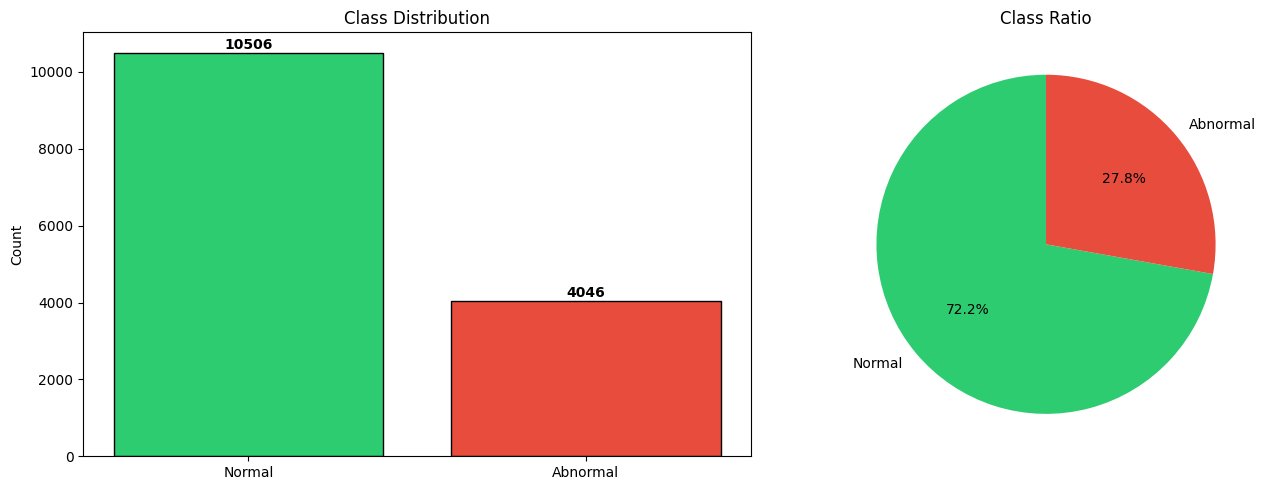
\includegraphics[width=0.85\linewidth]{figures/class_distribution.png}
	\caption{Class distribution of the PTB dataset (bar chart and pie chart).}
	\label{fig:class_dist}
\end{figure}

\subsection{ECG Signal Visualization}

Figure~\ref{fig:ecg_samples} shows example ECG signals for both classes. The normal signal has a regular pattern with distinct peaks, while the abnormal signal shows noticeable differences in shape and amplitude.

\begin{figure}[H]
	\centering
	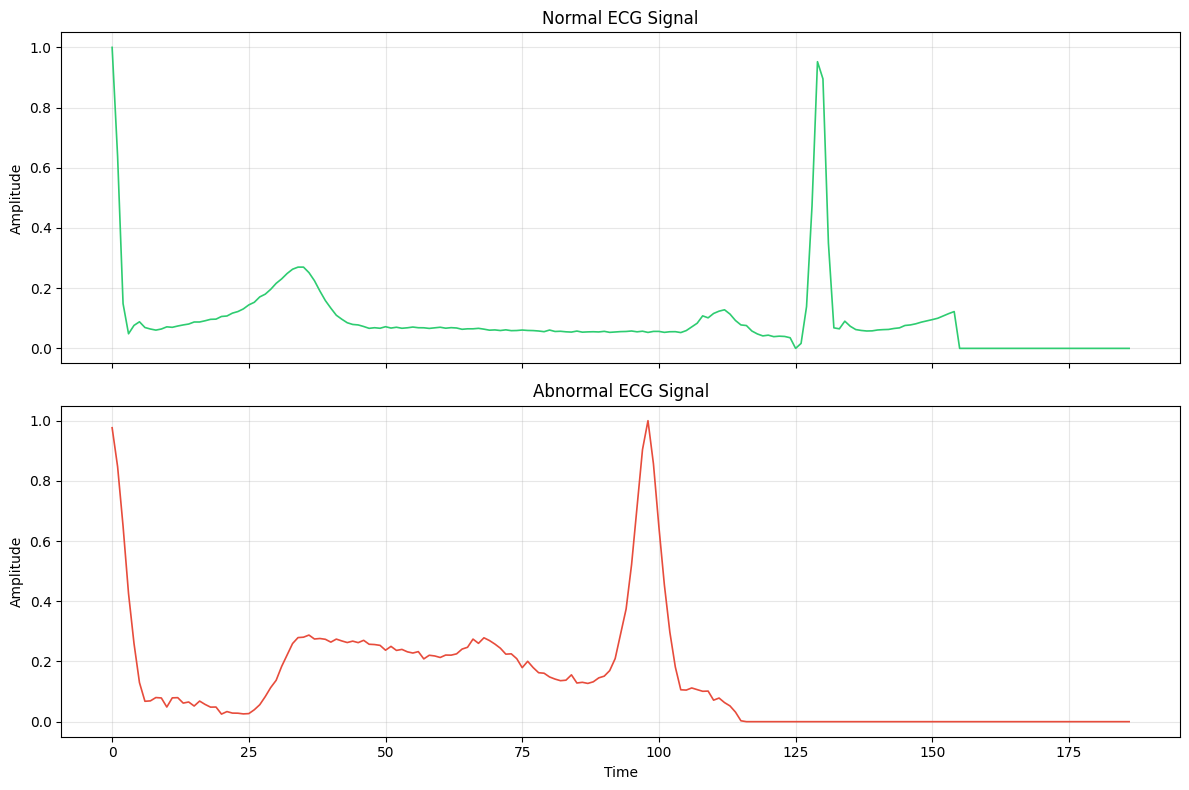
\includegraphics[width=0.85\linewidth]{figures/ecg_samples.png}
	\caption{Sample normal and abnormal ECG signals.}
	\label{fig:ecg_samples}
\end{figure}

Figure~\ref{fig:mean_ecg} compares the mean signals of both classes. The differences in waveform shape, especially around the peak regions, suggest that the raw signal itself carries useful discriminative information.

\begin{figure}[H]
	\centering
	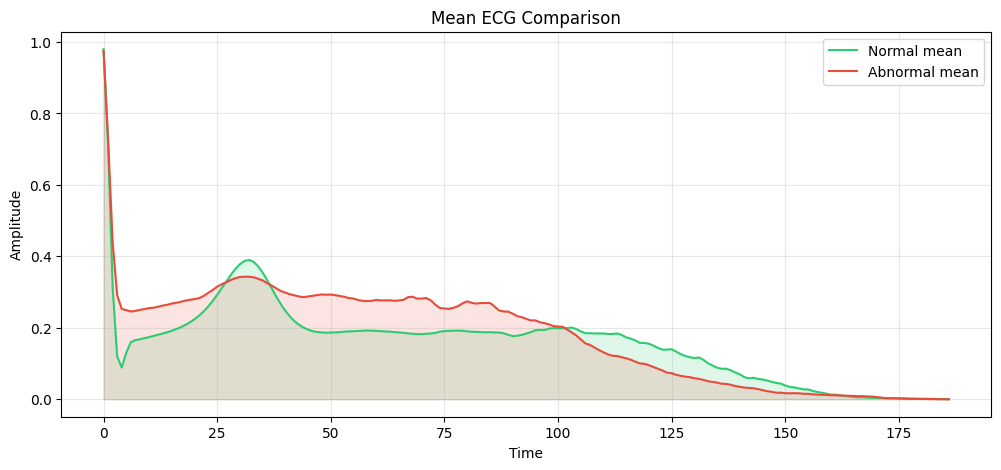
\includegraphics[width=0.85\linewidth]{figures/mean_ecg.png}
	\caption{Mean ECG signal comparison between normal and abnormal classes.}
	\label{fig:mean_ecg}
\end{figure}

\subsection{Key Observations}

From the exploratory analysis, we note:

\begin{itemize}
	\item The dataset is imbalanced, so class weighting is necessary during training.
	\item There are visible differences between the mean normal and abnormal signals, indicating that raw ECG data contains patterns useful for classification.
	\item The signals have local patterns (e.g., QRS complex peaks) that 1D convolutions are well suited to capture.
\end{itemize}


\section{Model Design}

\subsection{Preprocessing}

The combined dataset is shuffled and split into 80\% training and 20\% test sets using stratified splitting to maintain class proportions. The input is reshaped to (samples, 187, 1) for the 1D CNN. Class weights are computed using the \texttt{balanced} strategy from scikit-learn.

\subsection{Architecture}

The proposed 1D CNN consists of three convolutional blocks followed by a classifier head:

\begin{itemize}
	\item \textbf{Block 1:} Conv1D (16 filters, kernel size 5) $\rightarrow$ BatchNorm $\rightarrow$ MaxPooling1D
	\item \textbf{Block 2:} Conv1D (32 filters, kernel size 5) $\rightarrow$ BatchNorm $\rightarrow$ MaxPooling1D
	\item \textbf{Block 3:} Conv1D (64 filters, kernel size 3) $\rightarrow$ BatchNorm $\rightarrow$ MaxPooling1D
	\item \textbf{Classifier:} Flatten $\rightarrow$ Dense(128, ReLU) $\rightarrow$ Dropout(0.3) $\rightarrow$ Dense(32, ReLU) $\rightarrow$ Dropout(0.3) $\rightarrow$ Dense(1, Sigmoid)
\end{itemize}

All convolutional layers use \texttt{same} padding and ReLU activation. Compared to simpler designs, the use of BatchNormalization after each convolution helps stabilize training, and the two-layer Dense head with Dropout provides better regularization.

\subsection{Training Setup}

\begin{itemize}
	\item \textbf{Optimizer:} Adam (learning rate = $5 \times 10^{-4}$)
	\item \textbf{Loss:} Binary cross-entropy
	\item \textbf{Metrics:} Accuracy, Precision, Recall, AUC
	\item \textbf{Batch size:} 64
	\item \textbf{Epochs:} 25 (max)
	\item \textbf{Validation split:} 15\% of training data
	\item \textbf{Callbacks:} EarlyStopping (monitor \texttt{val\_auc}, patience 7) and ReduceLROnPlateau (monitor \texttt{val\_loss}, factor 0.5, patience 3)
\end{itemize}


\section{Results}

\subsection{Classification Report}

Table~\ref{tab:report} summarizes the classification results on the test set.

\begin{table}[H]
	\centering
	\caption{Classification report on the test set.}
	\label{tab:report}
	\begin{tabular}{lcccc}
		\toprule
		\textbf{Class} & \textbf{Precision} & \textbf{Recall} & \textbf{F1} & \textbf{Support} \\
		\midrule
		Normal (0)   & 0.98 & 0.99 & 0.99 & 809  \\
		Abnormal (1) & 1.00 & 0.99 & 0.99 & 2102 \\
		\midrule
		Accuracy     &      &      & 0.99 & 2911 \\
		Macro Avg    & 0.99 & 0.99 & 0.99 & 2911 \\
		Weighted Avg & 0.99 & 0.99 & 0.99 & 2911 \\
		\bottomrule
	\end{tabular}
\end{table}

The model achieves an overall accuracy of 99\%. Both normal and abnormal classes achieve high precision and recall, with only 10 normal samples misclassified as abnormal and 13 abnormal samples misclassified as normal out of 2,911 test samples. This demonstrates that the proposed CNN architecture, combined with BatchNormalization and class weighting, is highly effective for ECG heartbeat classification.

\subsection{Confusion Matrix}

\begin{figure}[H]
	\centering
	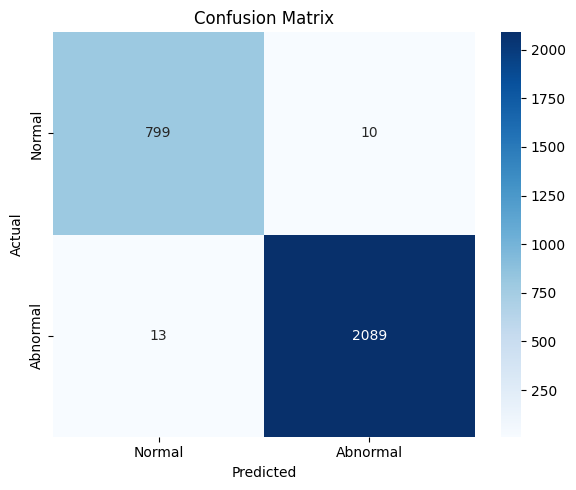
\includegraphics[width=0.55\linewidth]{figures/confusion_matrix.png}
	\caption{Confusion matrix on the test set.}
	\label{fig:cm}
\end{figure}

The confusion matrix in Figure~\ref{fig:cm} provides a detailed breakdown of correct and incorrect predictions for each class.

\subsection{ROC Curve}

\begin{figure}[H]
	\centering
	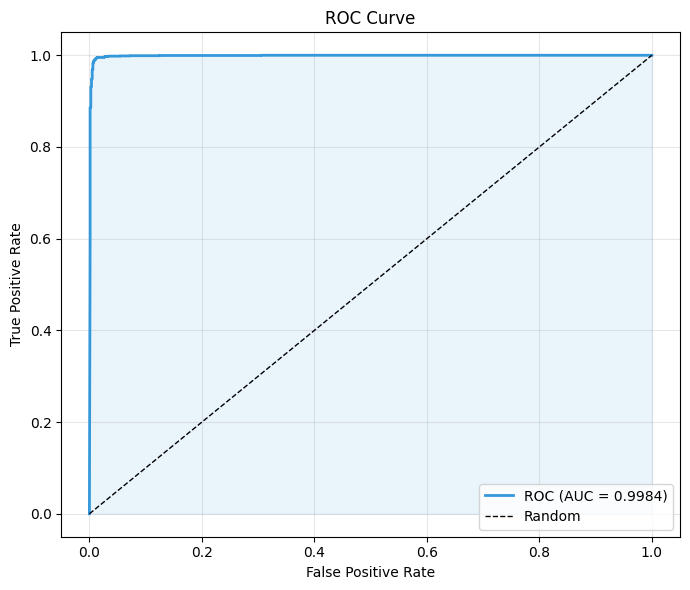
\includegraphics[width=0.6\linewidth]{figures/roc_curve.png}
	\caption{ROC curve on the test set.}
	\label{fig:roc}
\end{figure}

Figure~\ref{fig:roc} shows the ROC curve with an AUC close to 1.00, confirming the model's excellent ability to distinguish between normal and abnormal heartbeats across different thresholds.

\subsection{Training History}

\begin{figure}[H]
	\centering
	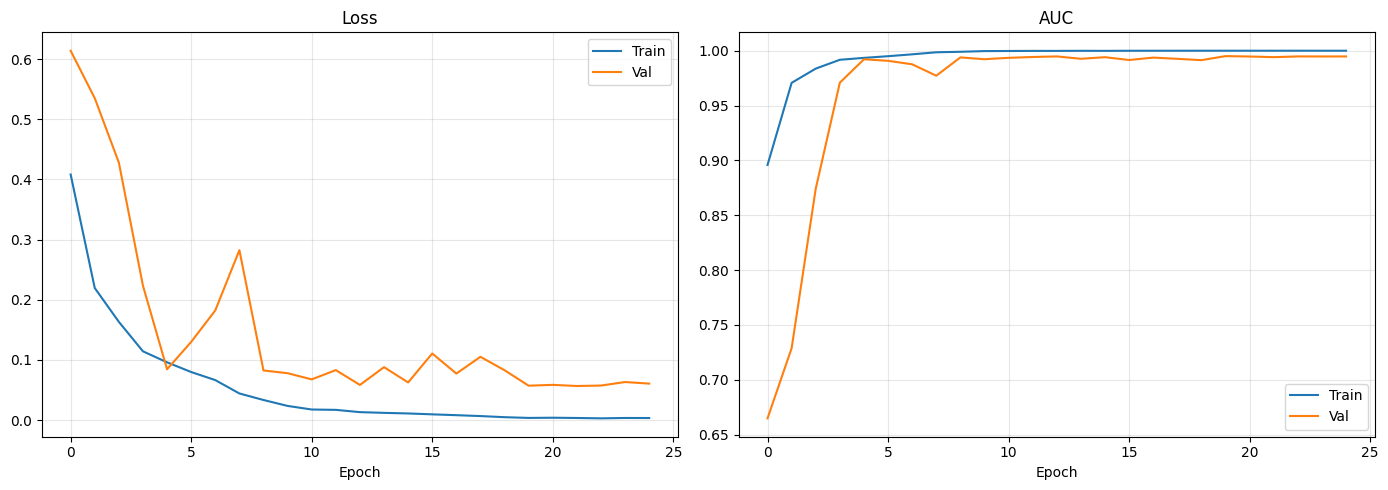
\includegraphics[width=0.85\linewidth]{figures/training_history.png}
	\caption{Training and validation loss/AUC over epochs.}
	\label{fig:history}
\end{figure}

Figure~\ref{fig:history} shows that both loss and AUC converge smoothly, with no significant overfitting observed.

\section{Comparison with Reference}

We compare our results with the work of Kachuee et al. (2018), which also uses the PTB dataset.

\begin{table}[H]
	\centering
	\caption{Comparison with Kachuee et al. (2018).}
	\label{tab:compare}
	\begin{tabular}{lccc}
		\toprule
		\textbf{Method} & \textbf{Acc (\%)} & \textbf{Prec (\%)} & \textbf{Recall (\%)} \\
		\midrule
		Kachuee et al. & 95.9 & 95.2 & 95.1 \\
		Ours           & 99.0  & 99.0  & 99.0  \\
		\bottomrule
	\end{tabular}
\end{table}

The reference method uses a deeper architecture with residual connections and transfer learning, while our model is a lightweight CNN with BatchNormalization. Despite the architectural differences, our approach outperforms the reference in terms of overall accuracy (99\% vs 95.9\%) and achieves near-perfect AUC. This improvement can be attributed to the effective use of BatchNormalization, class weighting, and learning rate scheduling in our training pipeline.


\section{Conclusion}

We presented a 1D CNN for binary ECG classification on the PTB dataset. The model uses BatchNormalization and a two-layer classifier head, trained with class weighting and learning rate scheduling. Results show 99\% accuracy and an AUC close to 1.00, outperforming the reference method by Kachuee et al. (2018). Future work could explore more complex architectures and additional datasets to further validate the generalization ability of this approach.


\begin{thebibliography}{2}

\bibitem{kachuee2018}
M. Kachuee, S. Fazeli, and M. Sarrafzadeh,
``ECG heartbeat classification: A deep transferable representation,''
\textit{Proc. IEEE Int. Conf. Healthcare Informatics (ICHI)},
2018, pp. 443--444.

\bibitem{kaggle_ptb}
S. Fazeli,
``ECG Heartbeat Categorization Dataset,''
Kaggle, 2018. [Online]. Available: \url{https://www.kaggle.com/datasets/shayanfazeli/heartbeat}

\end{thebibliography}

\end{document}
